%!TEX root = ../../thesis.tex
%*******************************************************************************
%****************************** Design Chapter *********************************
%*******************************************************************************

\chapter{Design}

\ifpdf
    \graphicspath{{Chapters/Design/Figs/}{Chapters/Design/Figs/}{Chapters/Design/Figs/}}
\else
    \graphicspath{{Chapters/Design/Figs/}{Chapters/Design/Figs/}}
\fi
The design of software systems is a critical aspect of \ac{se}, as it determines how the system will function and how well it will meet the needs of its users.
The following chapter will detail the design and methodology used in the research and provide a thorough understanding of the research design and methods used in this study, and how it relates to the research question and objectives.
This chapter will discuss the solution design (see section \ref{design:section:soldesign}) which involves analyzing the problem by identifying the requirements and creating a detailed plan for how to address it.
Then, in the next section, we explain our tool (see section \ref{design:section:solutionconcept}) in terms of architecture, components, interfaces, and data models using the concrete requirements and solution approach developed in the previous section. 
This chapter will thoroughly explain the research design and methods used in this study and how it relates to the research question and objectives.
%********************************** % Solution Design **************************************
\section{Solution Design}
\label{design:section:soldesign}
In software development, solution design is a step in the software development life cycle that defines a detailed technical design for building the software solution.
This step is essential to ensure that the final solution meets the requirements and objectives and can be developed and tested efficiently.
To ensure that our study results can be applied to other contexts, we have created abstract design knowledge based on the \ac{dr} (see section \ref{design:section:designReqs}), codify our knowledge into \ac{dp} (see section \ref{design:section:designprinciple}) and the overall solution design.
%********************************** % Design Requirements **************************************
\subsection{Design Requirements (DRs)}
\label{design:section:designReqs}
Design requirements in \ac{dsr} are typically defined as a set of constraints and specifications that must be met by the design artifact to be considered a successful solution. 
These requirements can be functional, such as the specific features or capabilities that the design must have, or non-functional, such as performance, usability, or scalability.
To derive a solution, we define some \ac{dr}s with the help of the literature review and comparison of some tools.
In this context, each \ac{dr} refers to a generalized requirement that can be standardized and applied to future software applications. 
These requirements are abstract and cover a wide range of software needs.
We covered a wide range of topics including \textit{\ac{ui} Prototyping}, \textit{Low-Code/No-Code development}, \textit{Model-Based Software Engineering}, \textit{Continuous Experimentation}, \textit{Task-Based Usability Testing}, and the \textit{LEAN development process}.
The following section presents \textit{eleven \ac{dr}s} and their corresponding references in literature and tools.
% \paragraph*{Systematic literature reviews:} 
% Systematic literature reviews establish a solid basis for knowledge creation. 
% They help create theories and identify areas that require more research.
% By identifying existing literature and highlighting areas to explore, they also assist in the understanding of the problem space in DSR.
% Therefore, a comprehensive DSR project must include systematic literature reviews \cite{misc:dsr:webster}.
% \paragraph*{Interviews:}
% Interviews are regarded as empirical research to obtain primarily qualitative insights from individuals, such as specialists in a particular subject. 
% Suppose the interviewers are a part of the problem's stakeholder group.
% In that case, they may be utilized to establish requirements (or meta requirements) for the solution space that have a solid foundation for the problem space.
% For example, artifacts can be designed based on design principles (DPs) generated from interviews.
% Furthermore, the interviews can also be used to improve and evaluate the designed artifacts \cite{misc:dsr:mayring}. 
% \paragraph*{Other Methods:}
% Design requirements can also be generated using other methods or combinations of methods.
% Other methods include simulations, experiments, case studies, ethnography, and the grounded theory approach \cite{misc:dsr:nickerson, misc:dsr:varshney}. \\\\

\paragraph{\ac{dr}1: Heterogeneous Users} states that \textit{The product should support diverse users with different needs, goals, and capabilities and integrate internal and external users.} 
In literature, this is reasoned by the fact that different users may have different needs, preferences, and levels of technical expertise \cite{misc:lean:steve}.
By including a diverse group of users, you can get a broader range of feedback and insights into how the software performs for different users \cite{article:prototyping:weichbroth}, simultaneously reducing the biases among developers \cite{misc:lean:burmeister}.
In this context, the users can be from internal sources, such as employees, or external sources, like Amazon Mechanical Turk\footnote{Amazon Mechanical Turk: \url{https://www.mturk.com/}}.

\paragraph{\ac{dr}2: Iterative Refinement} states that \textit{The product should be designed and developed in an iterative, incremental approach with some continuous feedback mechanism.} 
In literature, this is reasoned by the fact that the iterative approach involves the idea of breaking down development into small, incremental cycles of work rather than trying to deliver a complete product all at once \cite{misc:lean:tutorial}.
The key benefit of an iterative approach is that it allows the development team to get feedback from users and stakeholders early in the development process and to make adjustments \cite{article:experiments:lindgren} to the product as needed.

\paragraph{\ac{dr}3: Interactive Design} states that \textit{User-friendly, frictionless, interactive and intuitive interfaces are essential for the software products helping the users improve the User Experience (\ac{ux}).} 
In literature, this is reasoned by the fact that a tool should have easy navigation \cite{article:prototyping:hoffnagle}, clear and concise labels, icons, easy-to-use drag-and-drop functionality, collaboration capabilities (e.g., Figma\footnote{Figma Prototyping tool: \url{https://www.figma.com/}} has a feature where more than one person can access the prototype), reviewing and refinement \cite{paper:prototyping:luqi} features.
Various live examples like Figma, Invision\footnote{Invision: \url{https://www.invisionapp.com/}}, Axure\footnote{Axure Rapid Prototyping: \url{https://www.axure.com/}} have shown how user-friendly, interactive and intuitive tools have an impact on the users and improve the product.

\paragraph{\ac{dr}4: Engage Stakeholders} states that \textit{Various stakeholders (e.g., designers, product managers, developers, etc.) must contribute to the quick development of the product.}
In literature, this is reasoned by the fact that involving different project stakeholders and providing them with the necessary communication tools helps exchange and codify knowledge \cite{article:prototyping:weichbroth}. 
This makes sure that the stakeholders' perspectives, requirements \cite{misc:prorotypes:lauff}, and their input helps shape the product's design.

\paragraph{\ac{dr}5: Diverse Re-usable components} states that \textit{Collaboration between different team members and usage of the reusable components of various disciplines should make the tool easy for anyone to use on any platform and share their work quickly.} 
In literature, this is reasoned by developers' ability to create more consistent, user-friendly prototypes that adhere to the re-usable components' established style and principles \cite{paper:prototyping:luqi} and help improve the overall design process and product development \cite{article:prototyping:hoffnagle}.
In many tools, we saw the use of many reusable components like buttons, textbox, and other \ac{ui} components, data models for data transfer between components, and some guidelines to promote accessibility and usability of the tools.

\paragraph{\ac{dr}6: Enhanced Evaluation} states that \textit{The software product should be evaluated using various means by having users perform specific tasks, collect feedback, and improve the product.} 
In literature, this is reasoned by the fact that testing of the \ac{gui} of a software application is done using functional and usability tests \cite{misc:usability:tasks}. 
This helps the developers to identify any usability issues \cite{article:tbup:kari} and improve them continuously \cite{article:prototyping:gould}.
And this helps in the identification and preliminary validation of user requirements in the early stages of development \cite{article:prototyping:weichbroth}. 

\paragraph{\ac{dr}7: Improved Accessibility} states that \textit{The tool should be a web-based application making it accessible and independent of any software, platforms (e.g., Macbooks, Windows \ac{pc}s, Linux machines, Chromebooks) and have an auto-save feature to store the work on Cloud.}
In literature, this is reasoned by the fact that Web-based tools have several advantages \cite{misc:cloud} over traditional application-based tools.
In many tools like \texttt{Figma}, \texttt{Invision}, and \texttt{Axure}, we saw features\footnote{Some more features: \url{https://redrocksoftware.com.au/10-benefits-of-web-based-applications-systems/}} like \texttt{Accessibility} i.e., can be accessed from any device with an internet connection, \texttt{Collaboration} i.e., have built-in collaboration features, making it easy for team members to work on the same prototype simultaneously, \texttt{Updates} i.e., automatically updated.

% \textbf{DR9: Get user feedback} \textit{} Having users perform specific tasks and observe how they interact with the application helps improve the usability of the software applications. So, we can use task-based usability testing for achieving this. 
\paragraph{\ac{dr}8: Combined feedback} states that \textit{The software product should gather user feedback and combine them to make improvements to the application.} 
In literature, this is reasoned by the fact that \texttt{Qualitative analysis} gathers an in-depth understanding of underlying reasons, opinions, and motivations \cite{misc:dsr:mayring}.
Whereas \texttt{Quantitative analysis} measures and understands numerical data and helps identify patterns and trends \cite{article:qqa:young}.
And together, qualitative and quantitative analysis can provide a more complete picture of a situation and can be used to validate or disprove findings from one type of analysis \cite{article:qq:helena}.

\paragraph{\ac{dr}9: Visualization} states that \textit{There should be a visualization tool for prototyping to help different stakeholders see and interact with the design and gather feedback.} 
In literature, this is reasoned by the fact that visualization helps in prototyping by allowing designers and stakeholders to see and understand the design in a way that is easy to understand \cite{article:comparative:prototypes}.
It also allows designers to identify usability issues \cite{article:prototyping:gould} early in the design process to make the end product user-friendly and easy to use.
In tools, various methods, like creating \texttt{Wireframes}, \texttt{Mockups}, and \texttt{Interactive prototypes}, are used for visualization.

\paragraph{\ac{dr}10 Quick delivery} states that \textit{A software product should be easily deliverable, reducing the complexity and deployment time and increasing the product's usability.} 
In literature, this is reasoned by the fact that when software is easy to build, development teams can be more productive and efficient, leading to lower development costs \cite{misc:lowcode:platforms} and can be quickly delivered. 
It's also easy for different development team members to understand and work on the code, thereby improving collaboration \cite{misc:prorotypes:lauff} and generating high-quality code.
Adding new features, scaling up, and making changes, as needed, make the tool more accessible and helpful \cite{article:prototyping:lowcode} to ensure that the product is developed and deployed with minimum effort \cite{article:prototyping:lowcode}.

\paragraph*{\ac{dr}11 Classified UI versions} states that \textit{A software product should be tested with various \ac{ui} versions or variants to analyze the best-fit variant for the product.}
In literature, this is reasoned by the fact that a product can be tested against different design solutions and variations \cite{article:CE:fitzgerald} to see which variant performs the best in terms of usability, aesthetics, and other characteristics \cite{article:controlled:experiements}. 
At the same time, continuously improve \cite{article:CE:ros} the product based on the feedback of the best-fit variant.

%********************************** % Design Principles **************************************
\subsection{Design Principles (DPs)}
\label{design:section:designprinciple}
Design Principles (DPs) are guidelines or rules used to guide the design process in \ac{dsr} \cite{misc:dsr:henver}. 
They provide a framework for making design decisions \cite{paper:designprinciple:gregor} and help to ensure that the final solution meets the goals and objectives of the research. 
\ac{dp}s are used for breaking down complex problems into smaller, more manageable parts.
This section codifies our knowledge during the design study and derives \ac{dp}s from abstract \ac{dr}s from the iteration cycle of the \ac{dsr}.
The following shows the \textit{Eight \ac{dp}s} and references to literature and tools that build the foundation for the mapped \ac{dr}s (see figure \ref{fig:design:table-drs-dps}). 
\begin{figure}[htbp!]
  \centering    
  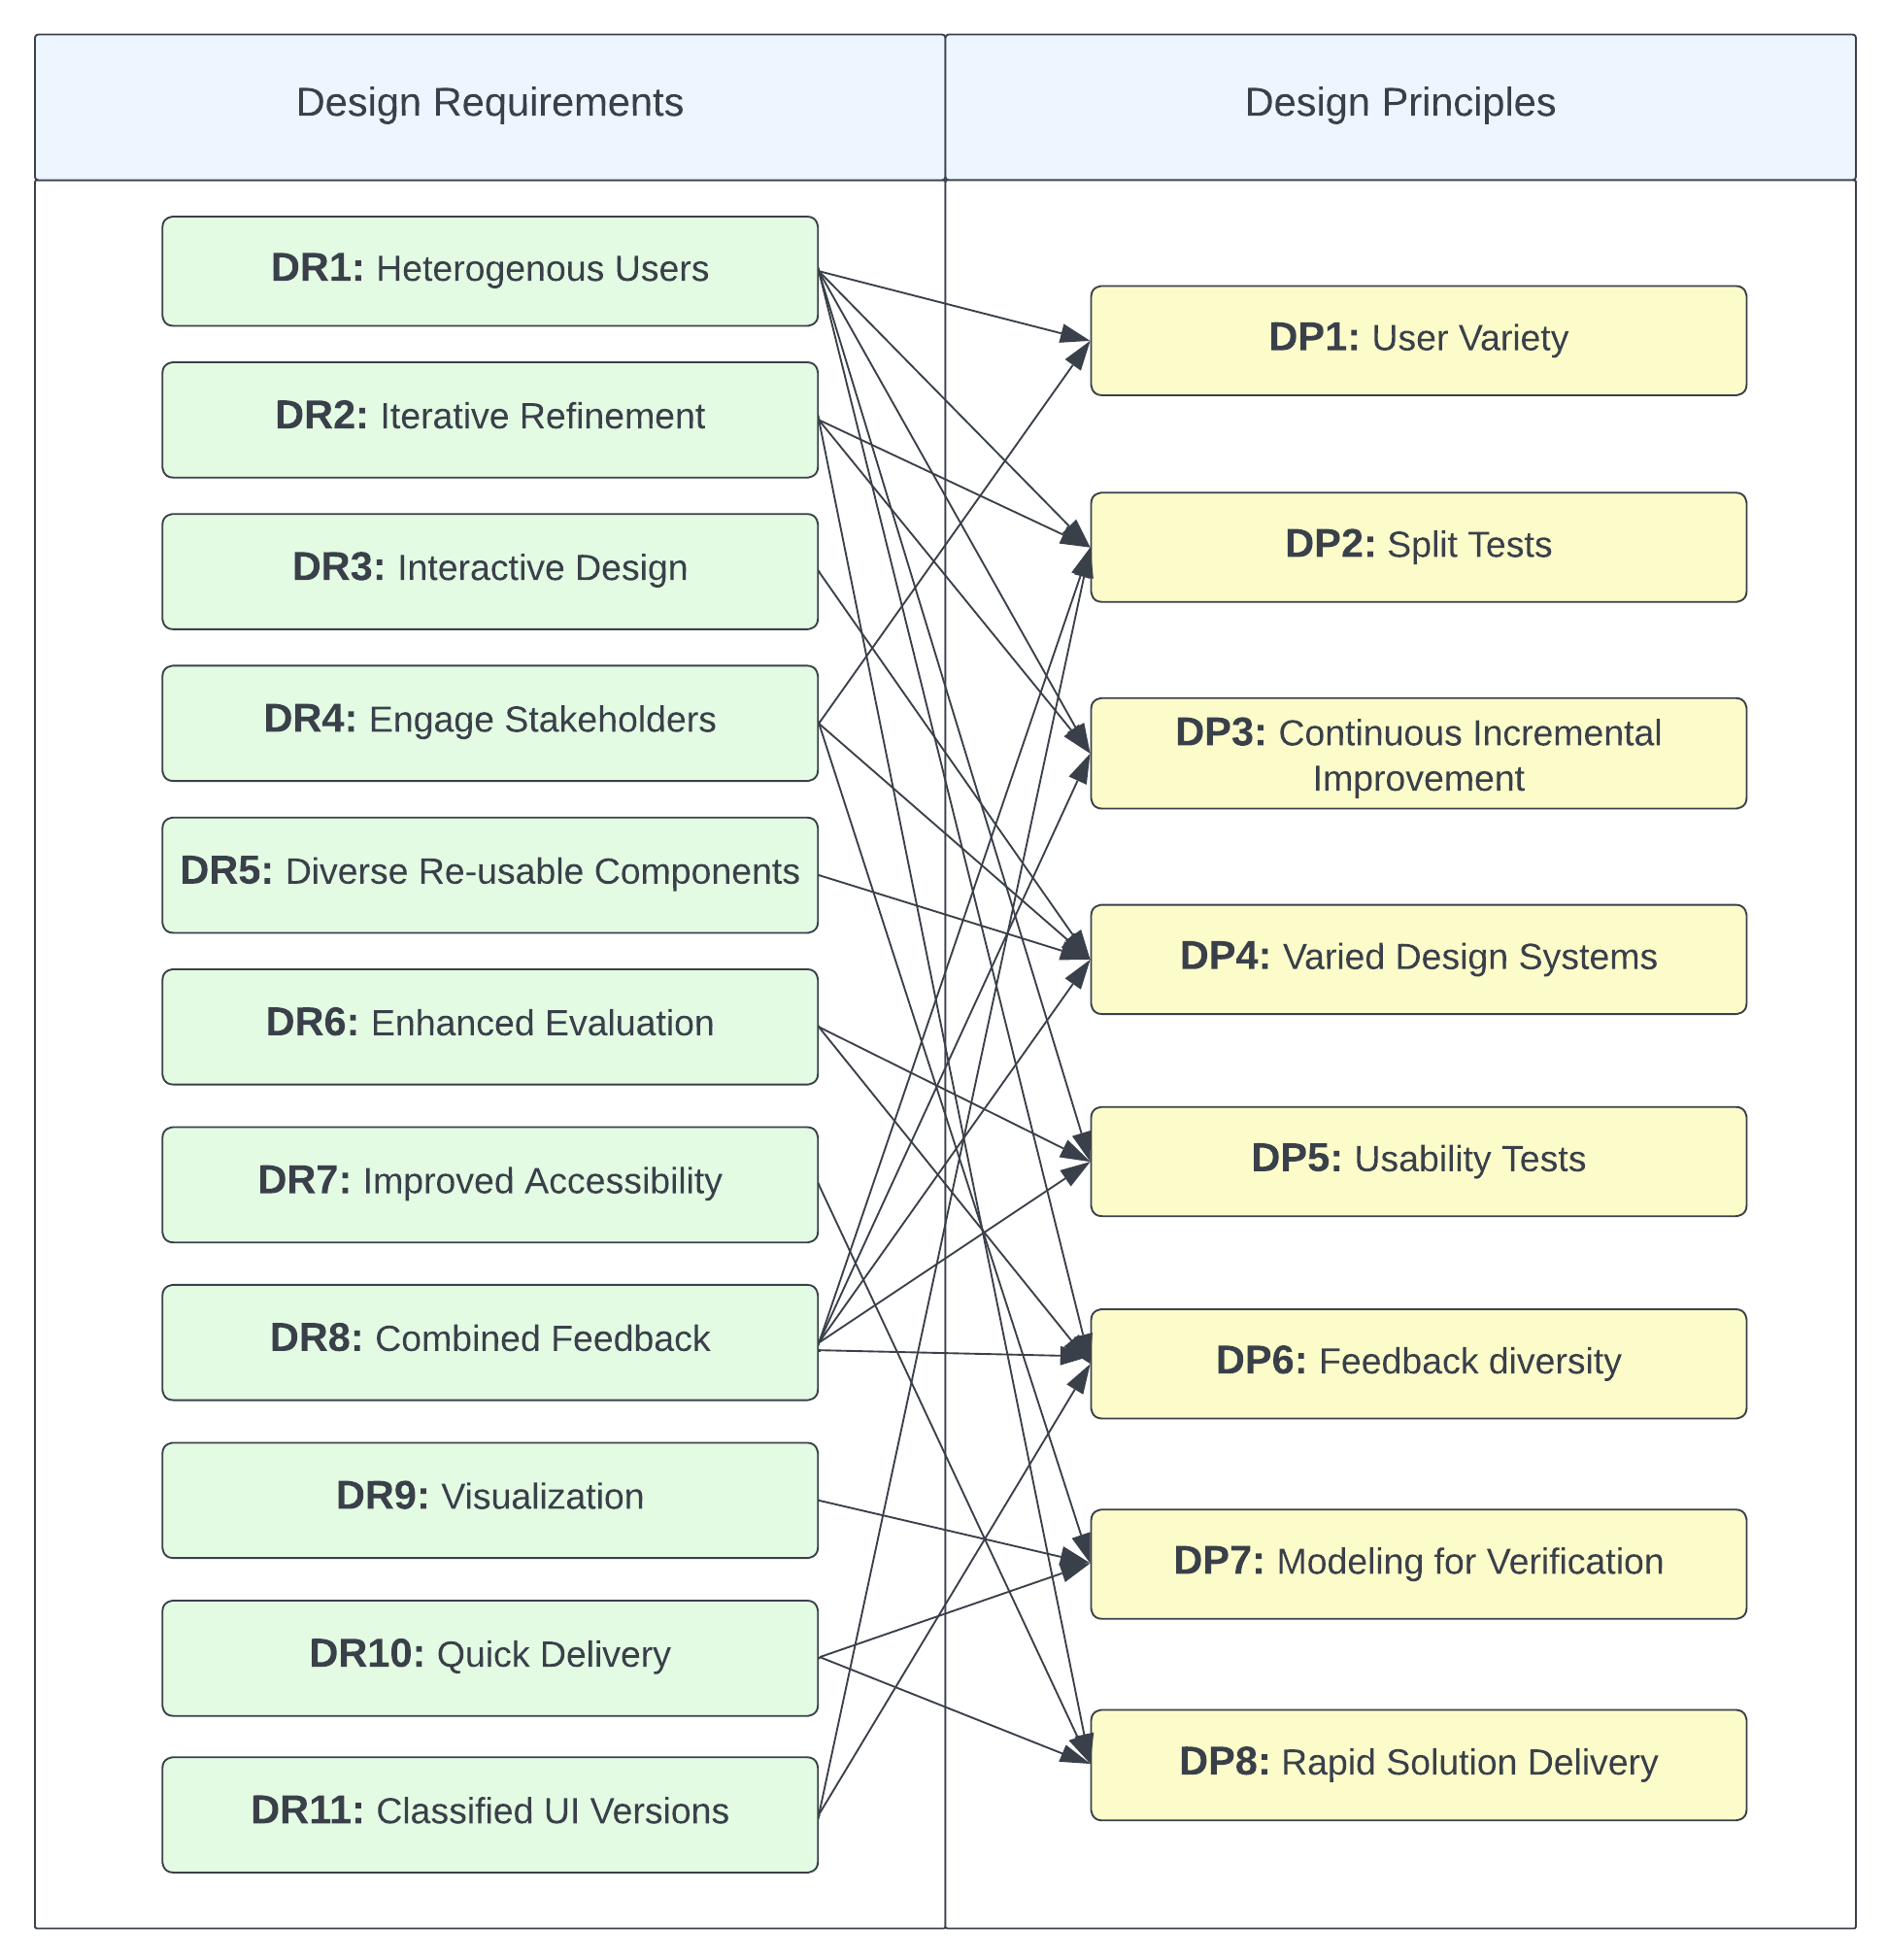
\includegraphics[width=0.86\textwidth]{Table-drs-dps.png}
  \caption[A map between \ac{dr}s and \ac{dp}s]{A map between Design Requirements and Design Principles}
  \label{fig:design:table-drs-dps}
\end{figure}

\paragraph{\ac{dp}1: User Variety:} \textit{Users with diverse requirements, objectives, and abilities should be able to use the product, and it should be able to accommodate both internal and external users within the organization.}

Developers have many unclear generalities early in the product development process \cite{misc:lean:steve} that they can clarify by testing the underlying assumptions using different types of users (i.e., \textit{DR1: Heterogenous Users}), and involving various product stakeholders (i.e., \textit{DR4: Engage Stakeholders}).
This helps to gather the user requirements smoothly, thus improving the product's usability.

\paragraph{\ac{dp}2: Split Tests:} \textit{Split tests can improve a software product by continuously testing different \ac{ui} versions or variants with shuffled users to get a winner or a best-fit variant from the users' feedback and improve the product.}

Split Tests (also known as A/B Testing) are performed on a randomly divided sample group of different users (i.e., \textit{DR1: Heterogenous Users}) by exposing each group to the \ac{ui} of different versions (i.e., \textit{DR11: Classified UI Versions}) to find out the feature that is most usable and functional for the users.
The results of the test are then used to determine which version is more effective by combining the feedback (i.e., \textit{DR8: Combined Feedback}) from the user groups and finally optimizing the whole product interatively (i.e., \textit{DR2: Iterative Refinement}).

\paragraph{\ac{dp}3: Continuous Incremental Design:} \textit{A software product broken down into minor, incremental phases in the software development process helps quickly improve software delivery and also helps to make product changes and improvements based on customer feedback.}

Using a continuous incremental approach, we can continuously improve software products by delivering value to customers as quickly as possible \cite{misc:lean:toyota}, constantly refining and improving the product \cite{misc:lean:planning}, and delivering the product as soon as possible.
Here, the iterative design should be used (i.e, \textit{DR2: Iterative Refinement}) to get continuous feedback from a variety of users (i.e., \textit{DR1: Heterogenous Users}).
The feedback which is collected should be a combination (i.e., \textit{DR8: Combined Feedback}) of various feedback helping significantly improve the application.

\paragraph{\ac{dp}4: Varied Design Systems:} \textit{A product should be developed using Design Systems innovatively by the citizen developers without complete reliance and dependence on the \ac{it} department.}

A \texttt{\ac{desy}}\footnote{Design Systems: \url{https://www.invisionapp.com/inside-design/guide-to-design-systems/}} is a collection of reusable components governed by some standards that can be assembled in many ways to make different applications.
A \ac{ui} Prototyping tool is helpful when different interactive (i.e., \textit{DR3: Interactive Design}) re-usable components are used as a drag-and-drop element (i.e., \textit{DR5: Diverse Re-usable Components}) while creating the prototypes by engaging various stakeholders' contributions (i.e., \textit{DR4: Engage Stakeholders}). 
It helps to get more feedback (i.e., \textit{DR8: Combined Feedback}) from the users or the customers, improving the product's usability and Functionality.
% In many tools, we saw the use of many \ac{desy} like \texttt{Design System Components} (e.g., buttons, forms etc.), \texttt{Design System Patterns} (e.g., patterns for communication and data transfer between components), \texttt{Accessibility standards} (e.g., some guidelines to promote accessibility).

\paragraph{\ac{dp}5: Usability Tests:} \textit{Usability testing can provide valuable insights into how users interact with a product and can help to improve the \ac{ux}. It's an effective method to detect usability issues early in the development process and to ensure the product is user-friendly, efficient, and easy to use.}

We can improve the usability of software by observing different users (i.e., \textit{DR1: Heterogenous Users}) as they interact with the product and measuring how well they can accomplish specific tasks or goals (i.e., \textit{DR6: Enhanced Evaluation}).
Moreover, the users can provide valuable insights into how easy or difficult it is to use the product and help identify areas where developers could improve the UI or design using user feedback (i.e., \textit{DR8: Combined Feedback}). 

\paragraph{\ac{dp}6: Feedback Diversity:} \textit{Diversity in software development feedback mechanisms helps ensure that a wide range of perspectives and experiences are considered when designing and testing software.}

Performing various tests (e.g., usability testing) with diverse users (i.e., \textit{DR1: Heterogenous Users}) ensures that the software is accessible and easy to use for different groups of people with an accurate evaluation of the task provided to the users (i.e., \textit{DR6: Enhanced Evaluation}).
Moreover, diversity in software development feedback mechanisms (i.e., \textit{DR8: Combined Feedback}), received by testing different UI versions (i.e., \textit{DR11: Classified UI Versions}), helps ensure the software is inclusive and accessible.

\paragraph{\ac{dp}7: Modeling for Verification} \textit{Modeling provides a clear and concise representation of the system being developed, thereby increasing communication among team members and stakeholders.}

A model-based approach increases transparency among various stakeholders, increasing their contribution to the product (i.e., \textit{DR4: Engage Stakeholders}) due to their excellent visualization capability (i.e., \textit{DR9: Visualization}).
Furthermore, modeling tools can automatically generate code or other documentation from the models, which can help reduce errors, improve efficiency, and decrease development time (i.e., \textit{DR10: Quick Delivery}).

\paragraph{\ac{dp} 8: Rapid Solution Delivery:} \textit{Rapid solution delivery in software development refers to the quick development and deployment of software solutions that meet the needs of users and stakeholders.}

We can achieve rapid solution delivery through the use of agile development methodologies and iterative design of the software (i.e., \textit{DR2: Iterative Refinement}).
With rapid solution delivery, software development teams can get feedback from users and stakeholders more quickly (i.e., \textit{DR10: Quick Delivery}) and adjust from the feedback increasing accessibility (i.e., \textit{DR7: Improved Accessibility}).

\subsection{Solution Design Concept}
\label{design:section:solutiondesign}
As shown in figure \ref{fig:design:solutiondesign},
\begin{figure}[htbp!]
  \centering    
  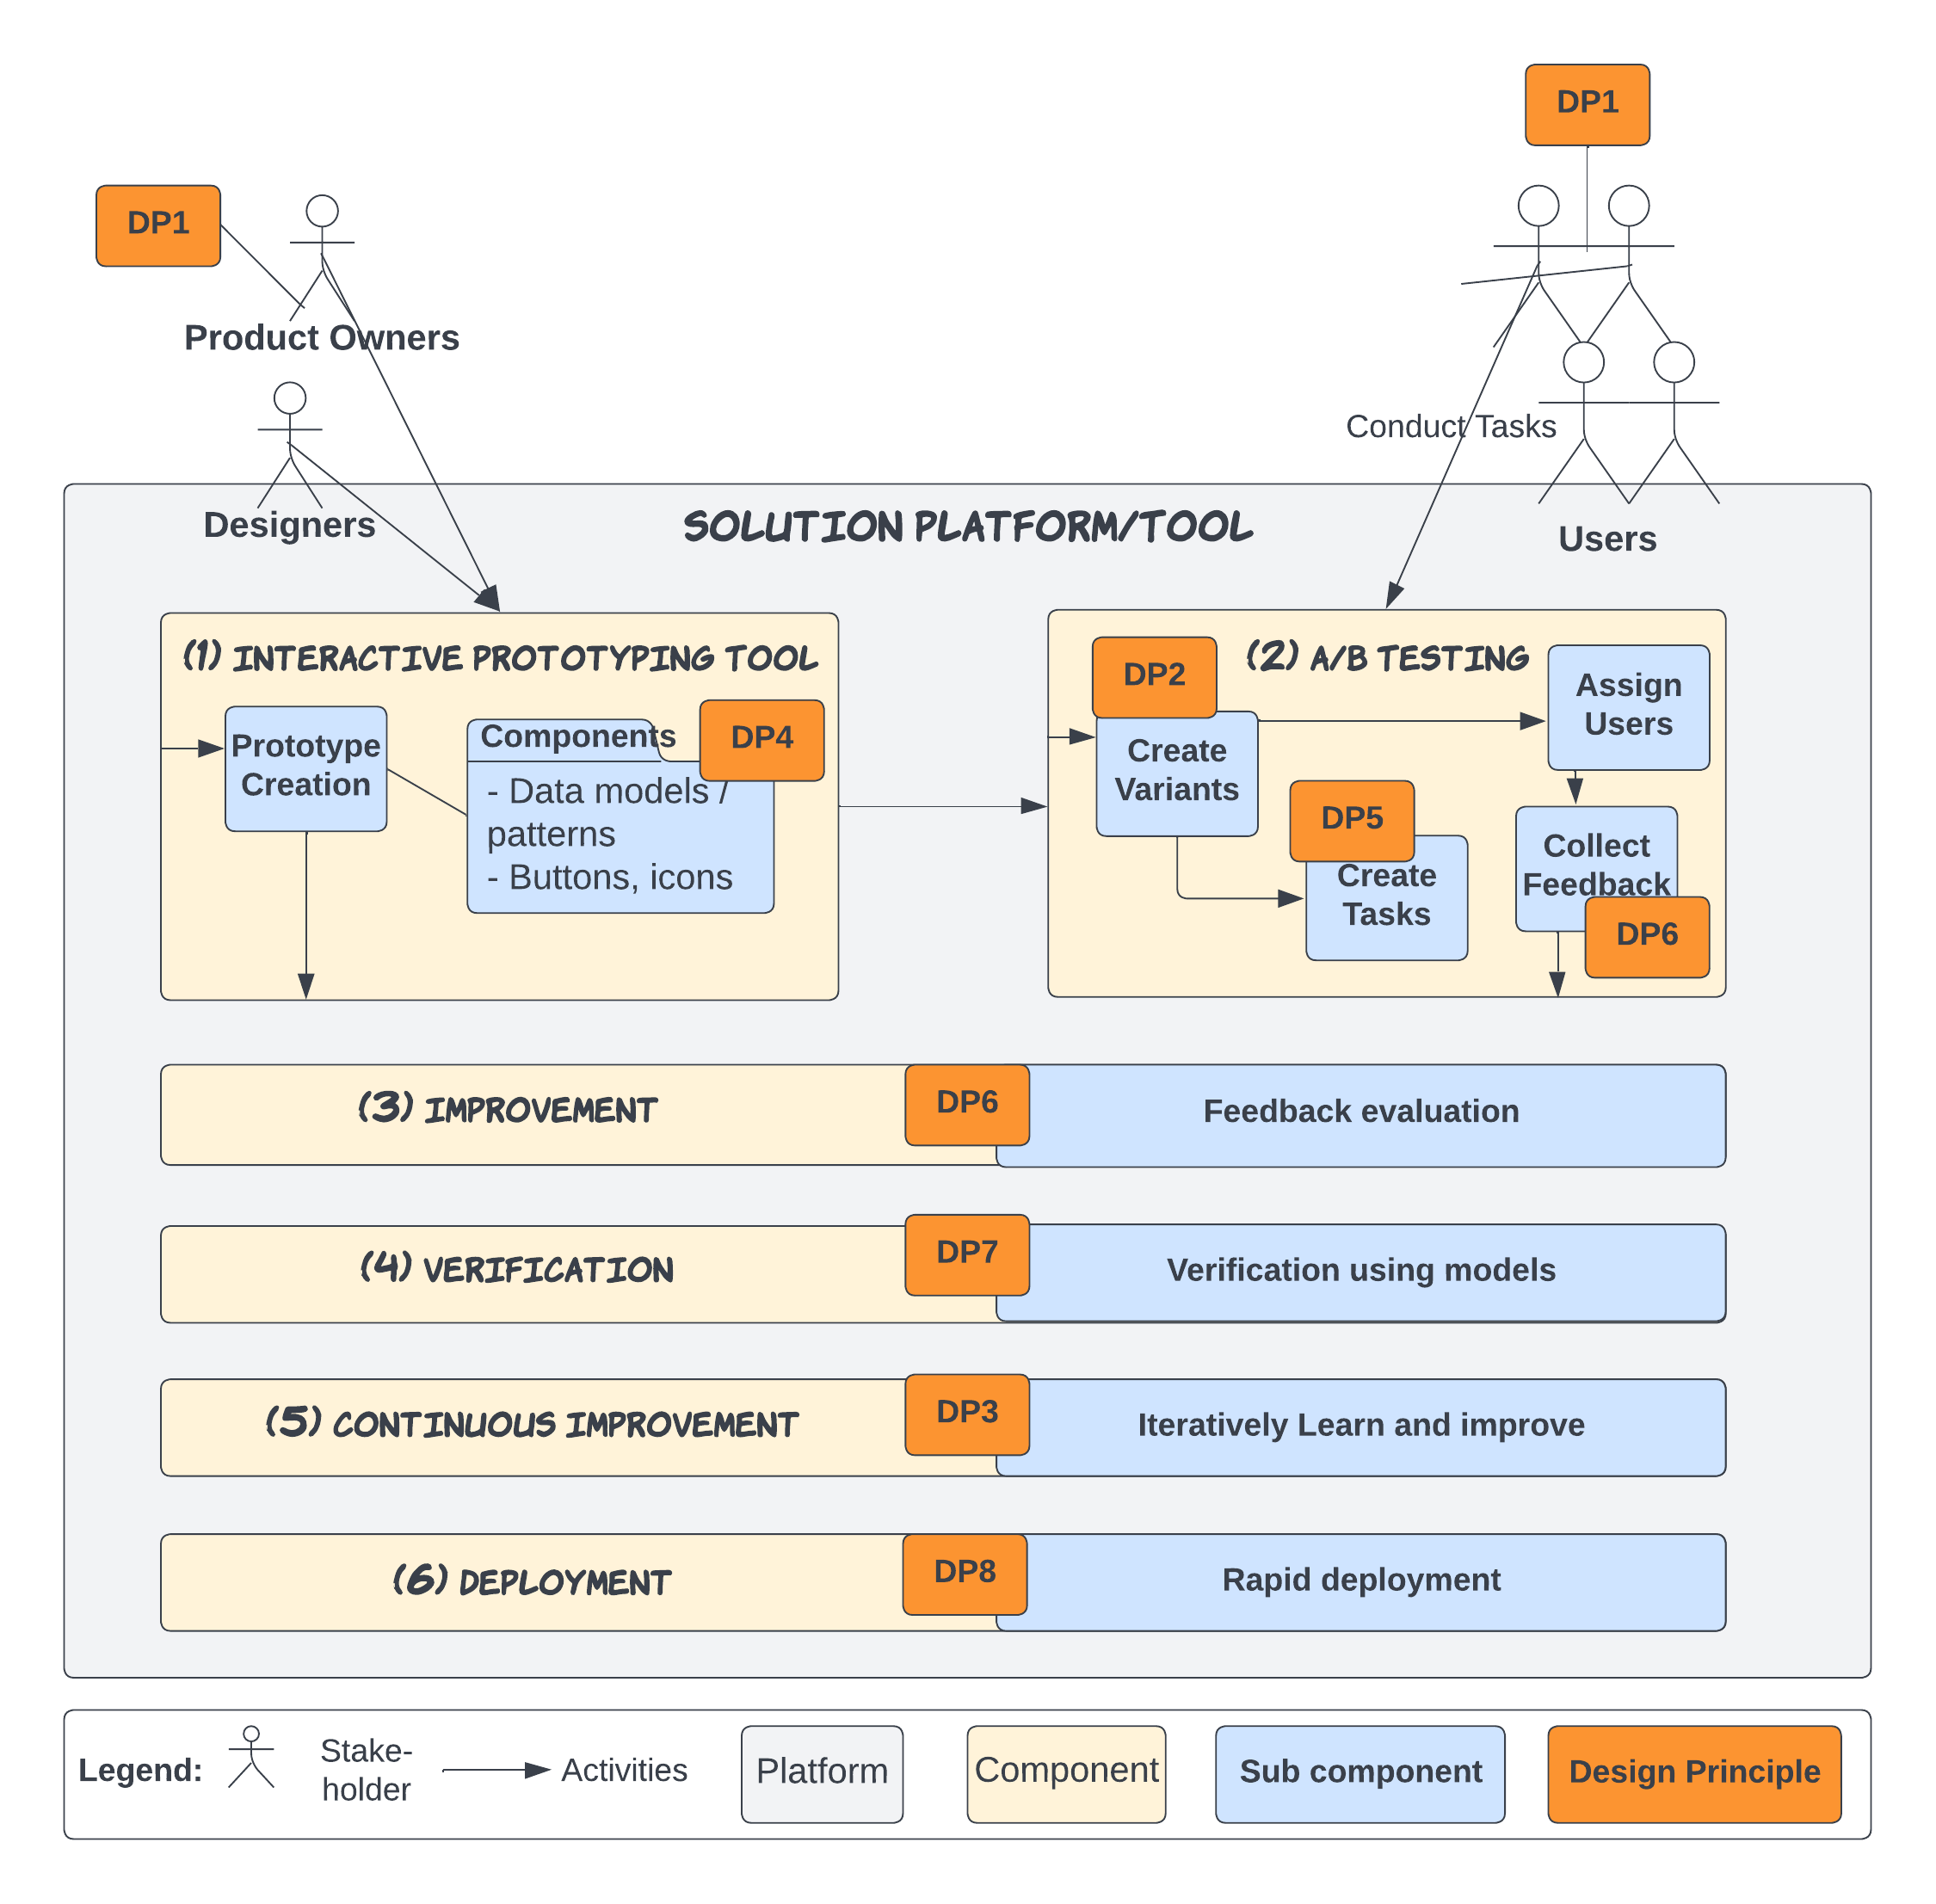
\includegraphics[width=0.9\textwidth]{Sol-design.png}
  \caption[Solution Design]{Solution Design for a UI Prototyping tool}
  \label{fig:design:solutiondesign}
\end{figure}

\clearpage
%********************************** % Solution Concept **************************************
\section{Solution Concept}
\label{design:section:solutionconcept}

\begin{figure}[htbp!]
  \centering    
  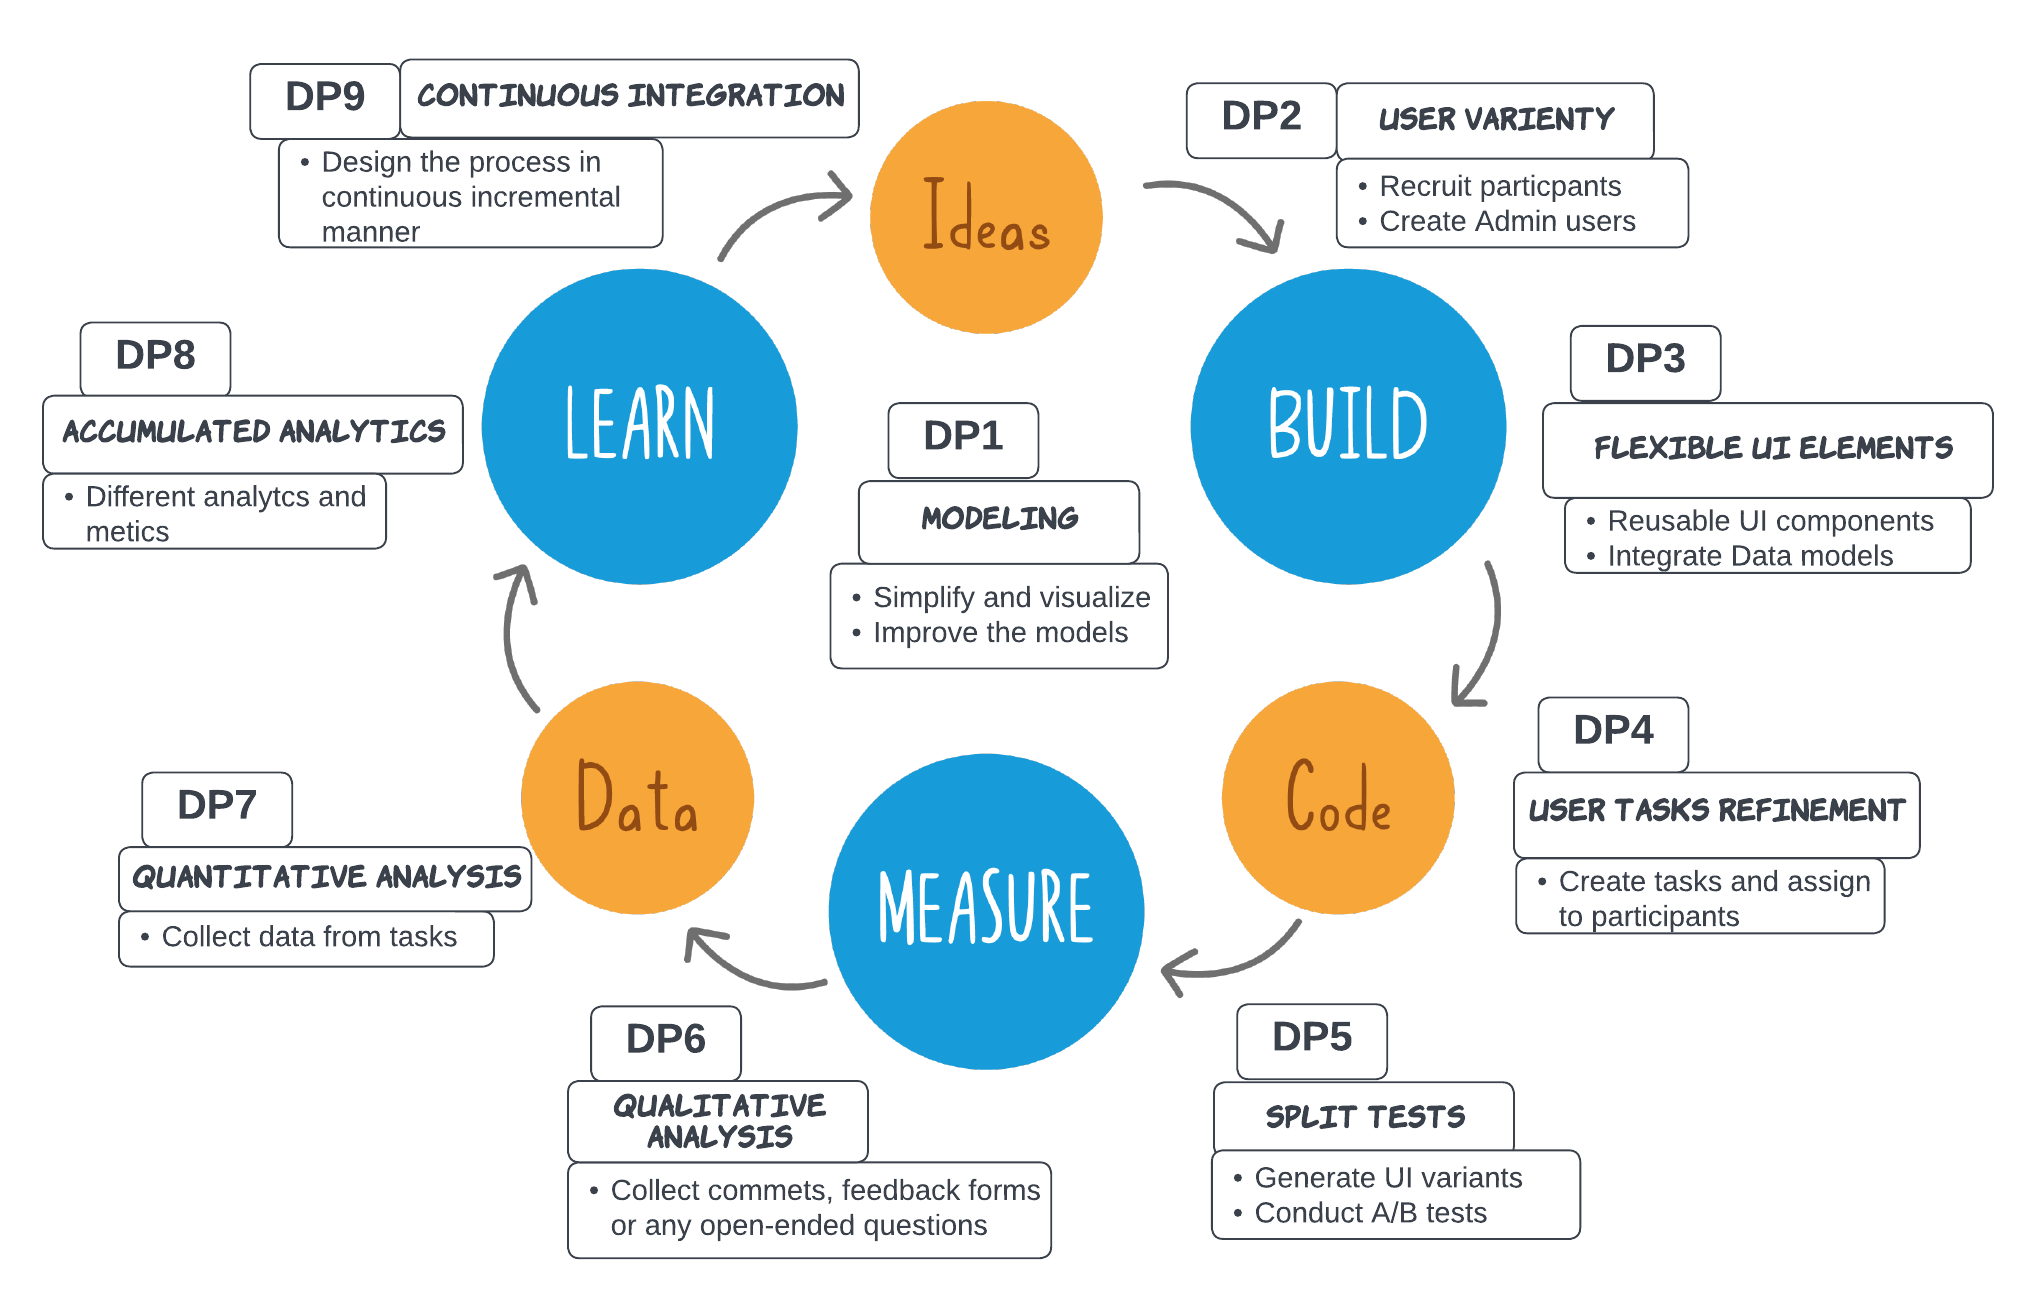
\includegraphics[width=0.6\textwidth]{LEAN-DPs.png}
  \caption[Solution Design]{Solution Design for a UI Prototyping tool}
  \label{fig:design:lean}
\end{figure}

%********************************** % Build **************************************
\subsection{Build}
\label{design:section:build}

%********************************** % Measure **************************************
\subsection{Measure}
\label{design:section:measure}
%********************************** % Learn **************************************
\subsection{Learn}
\label{design:section:learn}